% Activate the following line by filling in the right side. If for example the name of the root file is Main.tex, write
% "...root = Main.tex" if the chapter file is in the same directory, and "...root = ../Main.tex" if the chapter is in a subdirectory.
 
%!TEX root = testMain.tex

\chapter[Introduction]{Introduction}


When we find evidence for a hypothesis that we have held in the back of our minds, our belief in the hypothesis increases. This is the basic idea behind reasoning with evidence. In a constellation of hypotheses and pieces of evidence, we want to construct a network that will lead us to believe as many true hypotheses as possible, given the evidence that we have.

However, evidence itself is elusive, and its connection to hypotheses is as well - how can we be sure that some evidence supports some hypothesis? Even if we know that it does, how can we express how strong the piece of evidence is? Some evidence is very weak, and only after a tedious process of ruling out other factors and careful investigation and collection of other pieces of evidence, we can come to a conclusion about a hypothesis. On the other hand, some evidence is so strong that it leaves no room for doubt.

We all have intuitions about evidence strength - but can we make these intuitions precise? Additionally, can we manage the complex realities of weak evidence for many different hypotheses? 

\section{Bayes}

We have a way of expressing how we should use evidence to update our beliefs in hypotheses. We can do this with the use of probabilities. When we reason probabilistically with evidence, we want to use the gold standard - Bayes Law.
Let's say that we find some piece of evidence $e$, we want to know how our finding $e$ affects our belief in some hypothesis $h$. We can express how much we believe $h$ given $e$, using Bayes Law:

\[ P(h | e) =  \frac{P(e | h) \cdot P(h)}{P(e)}\]


This is the simplest form of Bayesian reasoning, one piece of evidence, and one hypothesis. But real life is not so simple, and we are constantly reasoning with many pieces of evidence. Small hypotheses can serve as stepping stones to greater hypotheses. One way of handling the complexity of interacting pieces of evidence and hypotheses is by using Bayesian Networks.

A Bayesian Network is a directed, acyclic graph that represents the joint probability distribution over a set of events \citep{pearl1988}. BNs have nodes and arcs. Formally, the nodes are random variables that represent events. In case of our Bayesian Networks, these random variables represent hypotheses and pieces of evidence. An arc represent a conditional relationships between two nodes. Conditional probability is expressed in the conditional probability table (cpt) of every node. A node that is not conditionally dependent on any other node (has no incoming arcs) is independent. 

 An example of a Bayesian Network can be seen in Figure~\ref{exampleBN}. It expresses a simple reasoning step: how should our belief in the hypothesis that our train will be late in Groningen, change once we learn about the train station renovations in Zwolle?
 
In the figure, the node `train\_on\_time\_in\_groningen' is a hypothesis. Nodes with one or more incoming arcs are conditionally dependent on their parent node(s). In our example network, the node `station\_renovation\_zwolle' is conditionally dependent on its parent. The links between the nodes are links of conditional probability, and do not correspond to real-world causality, although they are sometimes interpreted as being causal \citep{Dawid2008}.

\begin{figure}[h]
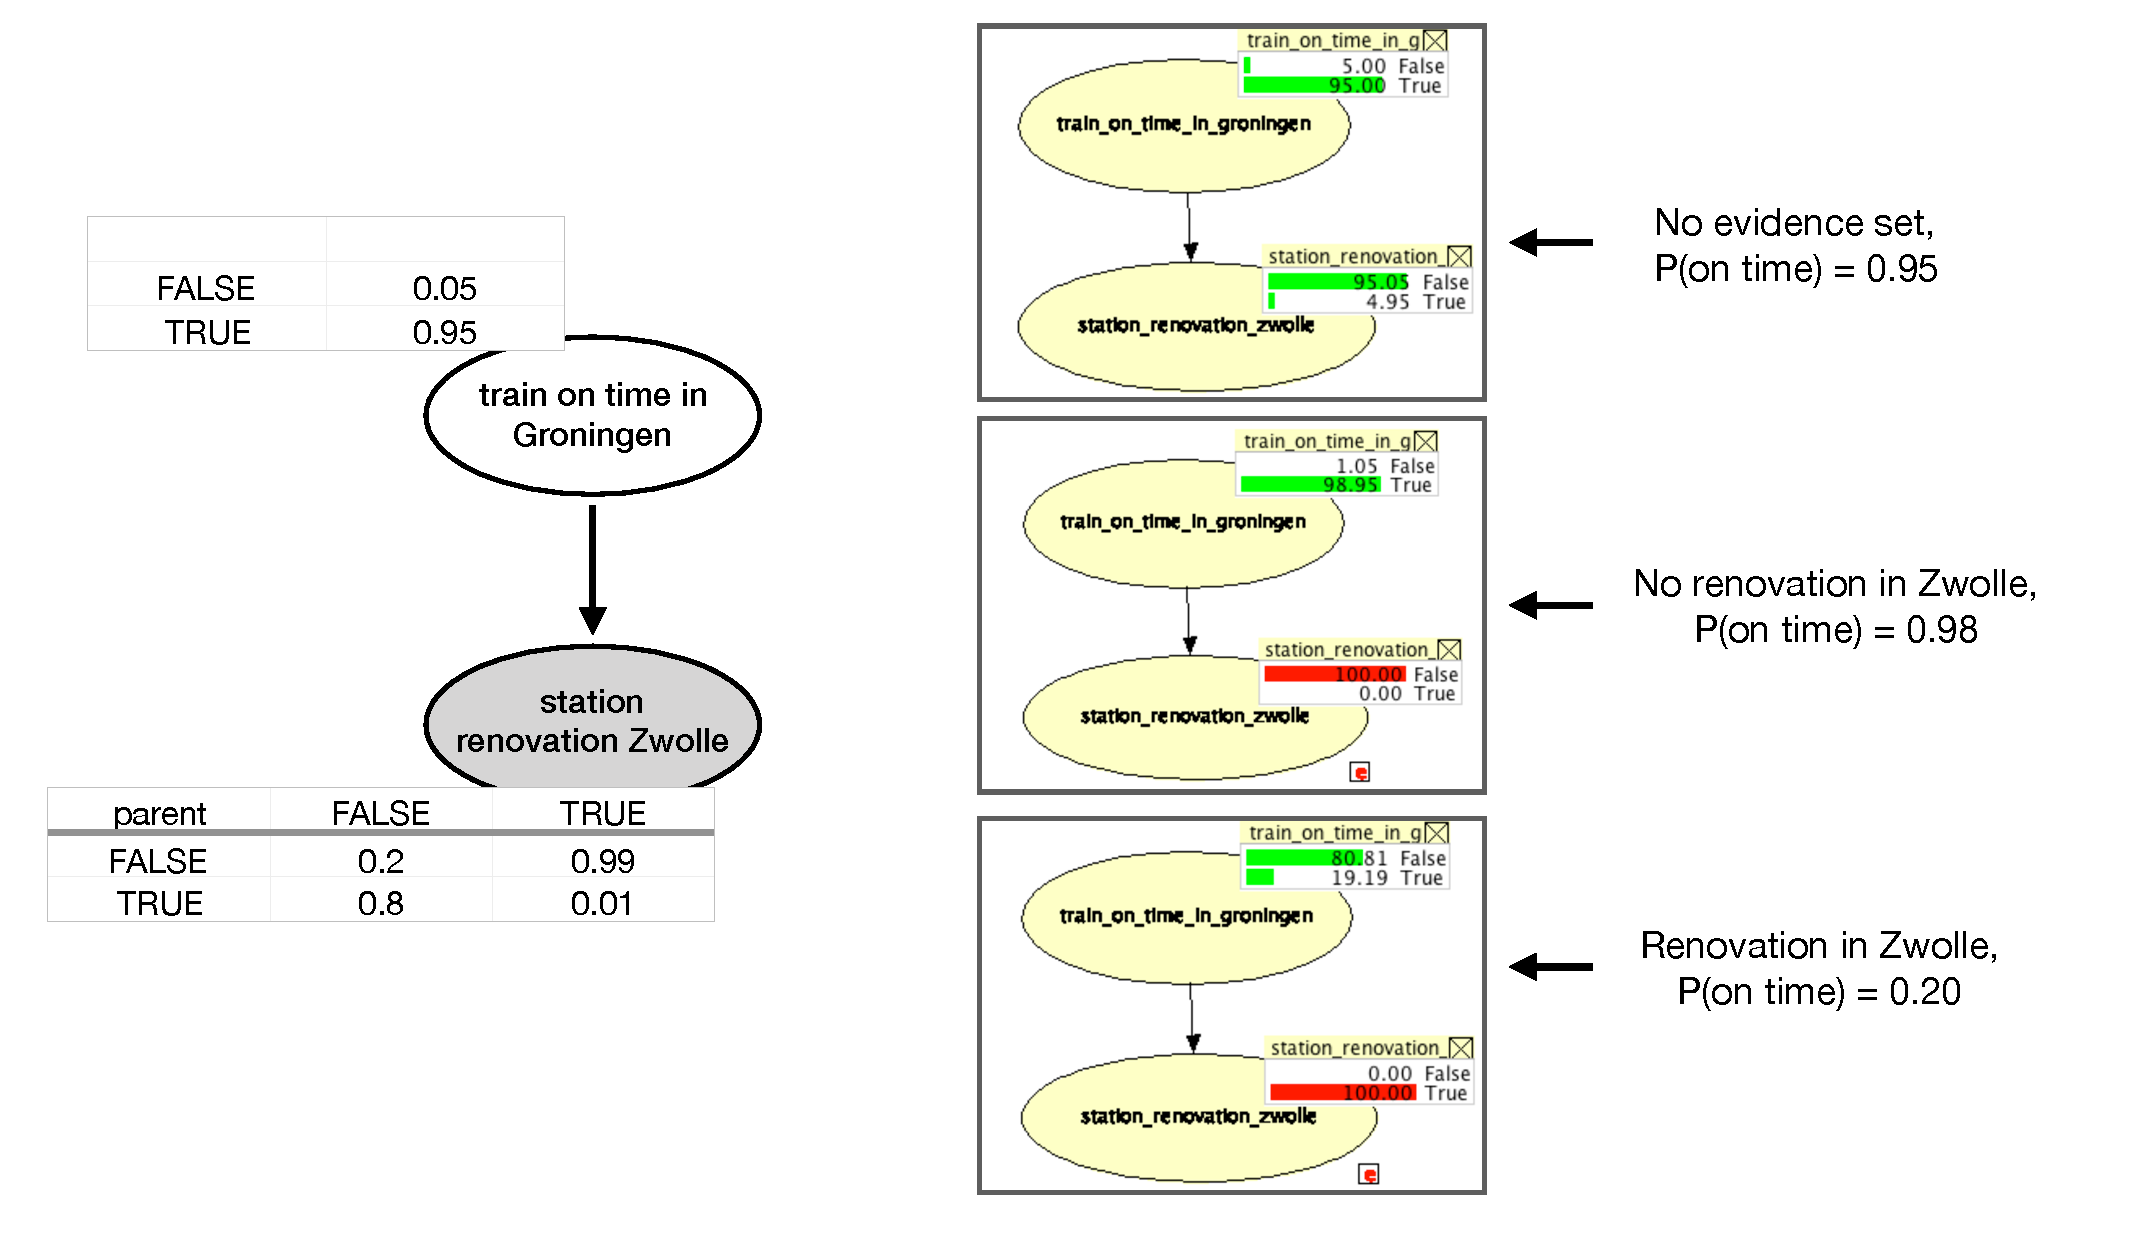
\includegraphics[width=\linewidth]{images/bnExample.pdf}
\caption{An example of a Bayesian Network, with and without evidence set.}
\label{exampleBN}
\end{figure}

We can reason with Bayesian Networks by setting evidence on one or more nodes that we can observe - our evidence. This means that we say whether some observable node is true or false, and use that information to update the network. We can now find a new posterior probability for a node that we cannot observe directly (yet). In Figure~\ref{exampleBN}, this means that when we learn that there are station renovations going on at Zwolle, the our belief that our train will be late in Groningen increases from a probability of 0.01, to a probability of 0.8. 

\section{This project}
Using Bayesian Networks, we can make explicit how we think that we should reason about hypotheses given pieces of evidence. In our toy example, this is not very consequential, it is a very simple network. However, Bayesian reasoning and Bayesian Networks specifically, can be applied to many domains. One of which is AI and law, specifically, Bayesian Networks might be tools that could be useful in court cases, by organising evidence and hypotheses. A Bayesian Network might make explicit how reasoners should update their beliefs based on the evidence, which might increase transparency and fairness. In the ideal case, a Bayesian Network might stop a judge from making a reasoning error!

However, creating Bayesian Networks is very complex, especially in domains where probabilistic data is sparse. We also do not have a good idea if our methods for creating Bayesian Networks in criminal situations work, since it is difficult to test these networks empirically - you cannot ask a murderer to murder again, for the statistics. This is why we need a grounding to investigate whether our methods for building Bayesian Networks actually work.

This is why this project proposes to ground Bayesian Networks for crimes in multi-agent simulations of crimes. We can model crime cases using simulations to a level of realism we desire. We can see what probabilities emerge out of these simulations by running them multiple times, and see if we can capture this probabilistic information into Bayesian Networks. We can collect exactly the frequency information that we need. This means that we can focus on assessing the Bayesian Networks, since we know what frequency information they should replicate.

\subsection{Research Questions}
\begin{itemize}
\item \textbf{Can we create Bayesian Networks that correctly reflect multi-agent simulations of crimes?}
\item \textbf{If we can, under what assumptions do these networks function?}
\end{itemize}



\section{Overview of the thesis}
Chapter 2 is an overview of the state of the art, Chapter 3 proposes a pipeline for creating simulations and automatic Bayesian Networks, and evaluation criteria that state when a Bayesian Network correctly reflects multi-agent simulations of crimes. Chapter 4, 5 and 6 are applications of this pipeline in three separate simulations: first a simple, non-spatial simulation based on \citep{Vlek2015}, a simple spatial simulation of a home-robbery, and finally a spatial simulation of a street-robbery. For each of these simulations, some simple experiments are done to investigate several problematic aspects of Bayesian Networks. These simulations are then each evaluated based on the evaluation criteria set out in Chapter 3. Finally, we draw conclusions in Chapter 7. 

You can interact with the simulation in Chapter 6 on \url{https://shielded-journey-34533.herokuapp.com}.

Code for this project can be found at \url{https://github.com/aludi/simulationTest}.
